% !TEX root = ../main.tex
%==========================================%

\section{Introduction}\label{sec:Intro}

% \cite{harris2003trading}
%book value and fundamental value
%Volatility: tendency of having unexpected changes in the price. Reasons for price change: new information about values and the trader's wanting liquidity.
%Episodic volatility: large price change over a short period of time.
%Fundamental volatility (due to unanticipated changes)vs transitory volatility (due to trading activity by uninformed traders)
%Fundamental volatility: new information about a change in fundamental values is common knowledge, then price change happens without trading. If a few people know, price change is observed in high trading volumes.
%Fundamental volatility factors: for commodities, it is supply and demand affects. For currencies: national inflation rates, macroeconomic policies, trade and capital flows
%unexpected events cause fundamental price volatility
%commodities that are expensive to store are volatile.

% It is difficult to define a stable coin because, the more we read, it captures a negative sentiment (what a coin ought not to be) more than what a coin ought to be. It ought not to be like Bitcoin, whose volatility is high.

% Stablecoins are a topic of recent interest. A lot of blogs and some academic articles have systemized them. We know that the reader of this paper is expecting a chart of coins and what mechanisms they use: we do provide that, but we do not consider that the core contribution of the paper at all. Instead we really dug into finance to deeply understand the core methods and mechanisms that are employed for reducing volatility of a coin. We feel our paper is closer to a tutorial on stablecoins where we try to eliminate all the jargon (which is often misused and imprecisely applied) to explain the concepts, as well as drawing out appropriate foundations from finance.

% Example: if we described the approach of stable coin in two simple words: ``currency board'' and you need no further explanation (just, perhaps, some details on the parameters), this paper is not for you. If you have heard the term and have a vague sense of how it works, but couldn't really explain it or why it achieves stability, this paper is for you. If you have never heard the term, this paper is also for you.

% Two basic concepts: (1) a tokenization of a fiat currency (say a digital dollar) or any asset or asset portfolio of assets. This is an old idea: liberty reserve, eGold. (2) a low-volatility coin that is tied to any existing asset. For example, with USD as the baseline, Euros are much more stable than Bitcoin. It is not because Euros are backed by USD or have any direct reference to the USD. It is because USD and Euros use the same model, a central bank management, with similar inputs (the interest rates their customers, commercial banks, use when lending cash to each other to meet various legal requirements that help ensure the banks will have enough cash on hand to server their customers and can withstand some of their investments going bad without going bankrupt).

% Most of the coins are mostly focusing on the supporting infrastructure, maybe we also have to talk about the supporting infrastructure of the stablecoin
% Talk about the crypto custodianship somewhere in the paper
%==========================================%

\subsection{Motivation} %need a better name
\textblue{In this section we talk about volatility and what does stability mean, and we make argument that we're not economist and everything is explained in our own language}
Cryptocurrencies have gained a wide application after Bitcoin was first introduced in Satoshi Nakamoto’s (pseudonymous) 2008 whitepaper~\cite{nakamoto2008bitcoin}. For Bitcoin and any other cyptocurrency to function as money, they need to fulfill a set of properties that determine the strength and adoption of them \ie they are expected to serve as a medium of exchange, a unit of account, and a store of value. However, due to high fluctuations in their prices, majority of the cryptocurrencies do not meet these properties and hence they cannot be adopted as money~\cite{overview}.

Having said that, the volatile nature of cryptocurrencies (\eg Ether, Bitcoin) has raised the interest into what is known as stablecoin. Stablecoins (\ie cryptocurrencies with stable price) ensure that the fluctuation in the value remains low. Figure~\ref{fig:btcandfiat} illustrates the volatility of Bitcoin's value, when compared to fiat currencies, and the change of values of EUR, GBP, CAD, and BTC with respect to USD over time. Monthly values between January 2016 and November 2018 are shown. According the figures, while fiat currencies show stable behaviour, Bitcoin's value changes drastically over time, which makes it a non-stable cryptocurrency.

%========================%
\begin{figure}[!htb]
	\centering
	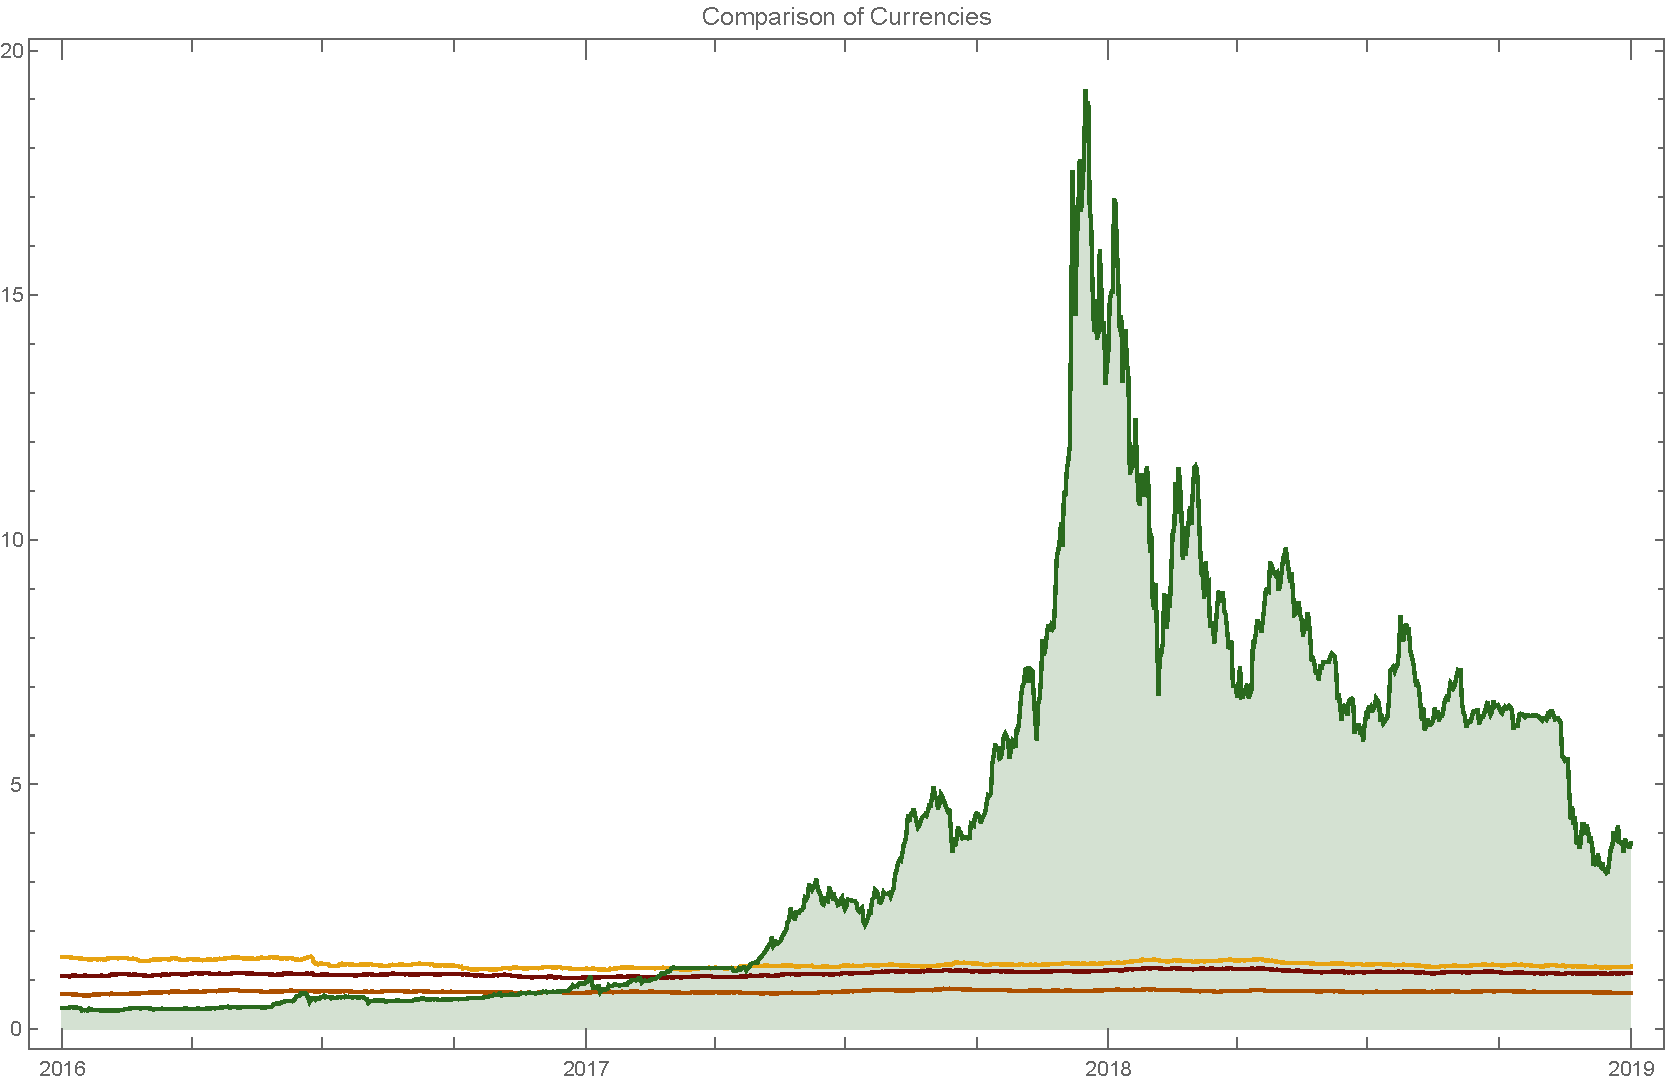
\includegraphics[width=0.75\textwidth]{figures/allCurrencies.pdf}
	\caption{\label{fig:btcandfiat}Comparison among fiat currencies and Bitcoin: The values are retrieved daily between  01-01-2016 and  01-01-2019.}
\end{figure}
%========================%


%========================%

\begin{figure}[!htb]
	\centering
	\subfloat[GBP with respect to EUR and USD]{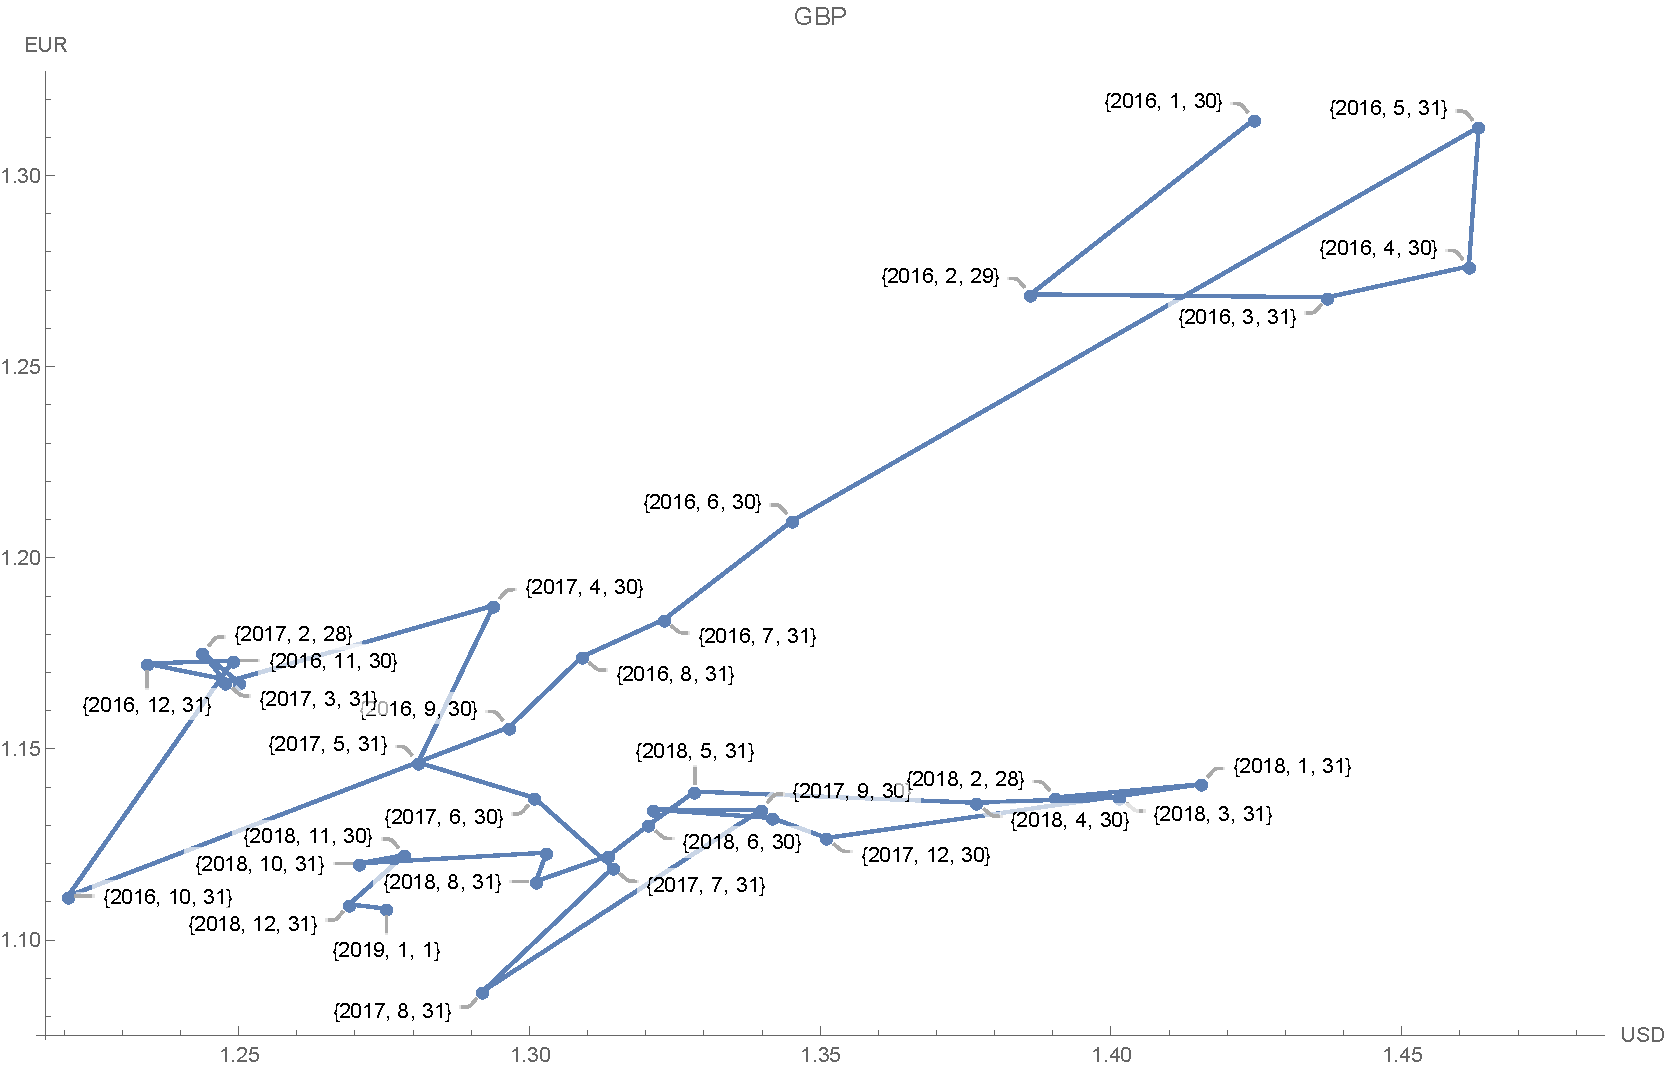
\includegraphics[width=0.75\textwidth]{figures/gbpBrexit.pdf}\label{fig:btc}}
	\hfill
	\subfloat[Legend]{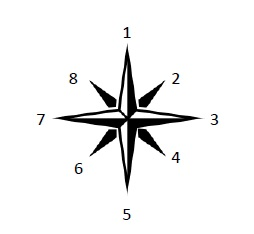
\includegraphics[width=0.25\textwidth]{figures/compass}\label{fig:legend}}
	\caption{Brexit's effect on GBP}
	\label{fig:Comparison}
\end{figure}
%========================%

%Figure1: It shows how extreme the volatility of BTC is, when compared to fiat currencies. 
% Prices retireved daily between 2016.01.01 and 2019.01.01
%EUR,CAD and GBP show stable behaviour.
%After June 23, 2016 (when the referendum for withdrawal of UK from EU took place), it can be observed that GBP and EUR values start to come closer as GBP loses and EUR gains value compared to USD. This is how volatility looks like in fiat currencies. Even such an important event with economical impacts didn't cause a high volatility compared to BTC price which exhibits more extreme changes in its value.

%Figure 2 illustrates GBP's behavior against EUR and USD. GBP plot moves in the 2-6 direction and there is a price drop of approximately 24 cents
%over a five month period following the referendum for Brexit. 
%Figure 2 zooms into the changes that GBP exhibits over time, as it is plotted over a small interval to reflect the price changes. Here Brexit's effect can be seen in more detail.
%Compared to Figure 1, the price drop is more visible, but it is worth noting that the price change is small compared to the changes in the value of BTC. NOTE: about terminology: price or vaue? or something different?
%GBP -(EUR and USD) chart "The pound dropped to its lowest level against the euro in 2017 after Mario Draghi, head of the European Central Bank, pushed the eurozone currency higher by saying he could start tightening monetary policy." September 2017 GBP loses value against both USD end EUR.


Figure~\ref{fig:btc} shows the change of value of Bitcoin with respect to USD and gold. The value changes happen in directions 2 and 6 (Figure~\ref{fig:legend}). The part of plot in direction 2 means that Bitcoin is gaining value against gold and USD. This can also be interpreted as both gold and USD are losing value relative to Bitcoin. %However, the first explanation is more likely to be the case, as only Bitcoin's value is changing compared to two values (USD and gold) changing.
Also, the fact that the plot is located on the diagonal shows that Bitcoin gains/loses value against both USD and Gold at the same time. This indicates that the changes in the values of USD and gold are highly correlated.

Considering these facts, there is a desire to design stablecoins with the stable nature of the fiat currencies together with the decentralized nature of the blockchain which is the underlying technology of cryptocurrencies.

%==========================================%
\section{Preliminaries}

\section{Related Works}
%Mahsa:





%==========================================%
%Didem:














%==========================================%
\subsection{Valuation}
% Every thing has two prices

%How do we assign value to something? how do we establish what something is worth?  The value is usually given in some units of account (\eg CAD).

%===Explaining the crossing===%

%When we establish a value for something, we do not really claim what the value is and what it worths, instead, we establish a value of its exchange. For example, today Alice is willing to pay 500 CAD for Bob's phone, whereas tomorrow, she will pay 600 CAD. What happened in this case? It could be (i) the value of money (CAD) going down or (ii) the value of good (phone) going up. Thus, in order to establish how much value something has, we should think of it in terms of being an exchange rate (the exchange rate between that asset and some other valuable assets). In other words, if Bob is willing to offer his phone for 1000 CAD, does it mean that it worths 1000 CAD? What we know about is that the value of Bob's phone is somewhere between 500 CAD (which Alice is willing to bid) and 1000 CAD (which Bob is willing to accept/ask). Therefore, the value of an object is not a single number and we can think of it as an interval between a least amount somebody wishes to sell for and the most amount somebody wishes to pay for that object, this interval is called bid-ask. If an ask comes below a bid, then the transaction happens and that amount is recorded as the final price, we call this \textit{crossing}.

%What actually happens when they cross? Assume that they cross in such that Bob wants to pay (bid) 600 CAD for Alice's phone while Alice wants to sell (ask) it for 500 CAD. What happens in the real world is (i) either one party goes first and advertises a bid or an ask and when it crosses with other party's complimentary bid or ask, she accepts it. (ii) both parties advertise and they do not know about each other's price, so when they cross, the market decides (usually they pick the midpoint between the two).

%When there is a cross, you have a price that is used for selling the object, that price is a last transaction price. So three values are actually important: 1) What is the most somebody is willing to pay for the object, 2) What's the least somebody is willing to accept for it, and 3) what was the last price this object is sold out. The value we see in the newspaper is always the last price, although it does not represent how much the object worths. In fact, we cannot actually say that and the best way to say that is when the bid-ask interval is really small. Assume that the interval is only 1 cent difference, in this case we can make sure what is the value and we are sure down to a cent. When the market changes so fast, the last price gives a lot of information on how much something worths, however, the last price that belongs to 30 years ago does not reveal a lot of information.

\subsection{Exchange}

\clearpage
\subsection{No-Seignorage Theory of Money}

To explain Bitcoin's exchange rate with fiat currencies, an oft-repeated theory has emerged that attributes Bitcoin's value to the hydro consumed by blockchain mining. While imprecise, the theory suggests that if a valuable resource $x$ is consumed to produce $y$, the value of $x$ is imparted into $y$. Setting aside the nuance that the hydro contributed to the Bitcoin system only indirectly produces new coins (it produces blocks, and blocks produce coins only for now), there is no economic principle underlying this transfer of value.

If Alice goes to Peter Luger's in Brooklyn, consumes a \$100 ribeye, and mints a literal shitcoin out of the result --- is that coin worth \$100 because it is ``backed'' by \$100 worth of steak?

\subsection{plot explanations}


%=======Plot Legend Explanation===========%
\begin{table}[t]
\centering
\begin{tabular}{|l|l|}
\hline
\textbf{Direction} & \textbf{Interpretation}   \\ \hline

         1/5                & $Y$ is losing (1) / gaining (5) value \\ \hline
         2/6                & Plotted asset is gaining (2) / losing (6) value \\ \hline
         3/7                & $X$ is losing (3) / gaining (7) value \\ \hline
         4/8                & \multicolumn{1}{p{12cm}|}{Plotted asset is gaining (4) / losing (8) value against $X$, while losing (4) / gaining (8) value against $Y$} \\ \hline

\end{tabular}
\vspace{1em}
\caption{\footnotesize{The interpretation of the plots.}\label{tab:plotlegend}}
\end{table}
%===================%



%==========================================%

\section{Systemization of stablecoins and Justification}

% Dollar tokenization vs. low volatitility

% !TEX root = ../main.tex


%-------------------Fancy Table ----------------------%

% = = = Rotated Table Entry \headrow


\newcommand{\headrow}[1]{\multicolumn{1}{c}{\adjustbox{angle=65,lap=\width-0.5em}{#1}}}

% = = = Table bullets: \full and \prt (full and part)

\newcommand{\full}{$\bullet$}
\newcommand{\prt}{$\circ$}
% ------------------------------------------------------------------------------------------------------------------------------------------------%
%Stablecoin projects%

\definecolor{UnitedNationBlue}{rgb}{0.30,0.53,1}
\definecolor{LightSteelBlue}{rgb}{0.69,0.77,0.87}
\definecolor{LightGrey}{rgb}{0.83,0.83,0.83}


\begin{table*}[t]
\centering

\begin{tabular}{|l|l|l|l|l|}

\hline
\rowcolor{lightgray}
\textbf{Class} & \textbf{Mechanism} & \textbf{Resembles} & Rank \\  \hline
% = = = = = = = = = = = = = = = = = = = = = = = = = = = = = = = = = = = = = = = = = = = = = = = = = = = = = = = = = = = = = = = = = = = = = = %
\multirow{17}{*}{Backed}		
						& \multirow{8}{*}{Directly-Backed \& Redeemable$^{\dagger}$}	& USDC 			& 20 \\ \cline{3-4}
						&													& TrueUSD 		& 26 \\ \cline{3-4}	
						&													& Paxos 			& 38 \\ \cline{3-4}		
						&													& Gemini Dollar 	& 52 \\ \cline{3-4}
						&													& StableUSD (USDS) & 685 \\ \cline{3-4}
						&													& Stronghold USD 	& 891 \\ \cline{3-4}
						&													& Petro 			& 1210 \\ \cline{3-4}
						&	& \multicolumn{1}{p{5cm}|}{Ekon, WBTC, emparta} & $\perp$ \\ \cline{2-4}
% = = = = = = = = = = = = = = = = = = = = = = = = = = = = = = = = = = = = = = = = = = = = = = = = = = = = = = = = = = = = = = = = = = = = = = %
						& \multirow{6}{*}{Directly-Backed}  							& Tether 			& 6 \\ \cline{3-4}
						&													& EURSToken 		& 95 \\ \cline{3-4}
						&													& BitCNY 			& 304 \\ \cline{3-4}
						&													& Terracoin 		& 1280 \\ \cline{3-4}
						&													& Saga 			& 1495 \\  \cline{3-4}
						&	& \multicolumn{1}{p{5cm}|}{GJY, Novatti AUD, UPUSD} & $\perp$ \\ \cline{2-4} 						
% = = = = = = = = = = = = = = = = = = = = = = = = = = = = = = = = = = = = = = = = = = = = = = = = = = = = = = = = = = = = = = = = = = = = = = %
						& \multirow{3}{*}{Indirectly-Backed}							& Dai 			& 57 \\ \cline{3-4}
                                                &													& BitUSD 			& 398 \\  \cline{3-4}
                                                & 													& Nomin			& $\perp$ \\ \cline{1-4}
% = = = = = = = = = = = = = = = = = = = = = = = = = = = = = = = = = = = = = = = = = = = = = = = = = = = = = = = = = = = = = = = = = = = = = = %
%						& \multirow{1}{*}{Market Manipulation} 						& NuBits			& 892 \\ \cline{1-4}
\multirow{5}{*}{Intervention}                                                           

% = = = = = = = = = = = = = = = = = = = = = = = = = = = = = = = = = = = = = = = = = = = = = = = = = = = = = = = = = = = = = = = = = = = = = = %
						& \multirow{2}{*}{Money Supply Adjustments}  				& Ampleforth		& $\perp$  \\ \cline{3-4}
						&   													& RSCoin 			& $\perp$  \\ \cline{2-4}
% = = = = = = = = = = = = = = = = = = = = = = = = = = = = = = = = = = = = = = = = = = = = = = = = = = = = = = = = = = = = = = = = = = = = = = %
						& \multirow{2}{*}{Asset Transfer}  							& NuBits			& 892 \\ \cline{3-4}
						&													& CarbonUSD		& 1262 \\ \cline{3-4}
						&													& Basecoin 		& $\perp$ \\ \cline{1-4}
% = = = = = = = = = = = = = = = = = = = = = = = = = = = = = = = = = = = = = = = = = = = = = = = = = = = = = = = = = = = = = = = = = = = = = = %
%						& \multirow{2}{*}{TBD: Internal }  								& Nautiluscoin 		& $\perp$ \\ \cline{3-4}
% = = = = = = = = = = = = = = = = = = = = = = = = = = = = = = = = = = = = = = = = = = = = = = = = = = = = = = = = = = = = = = = = = = = = = = %
\hline
\end{tabular}
\caption{Stablecoin proposals as of January 11, 2019. $\dagger$ \textit{Disclaimer:} Projects are classified according to what they assert; \eg we provide no warranty that projects classified as `redeemable' provide actual redemption of the assets that back their coins. Rank corresponds to \textit{CoinMarketCap}.\label{tab:stablecoins}}
\end{table*}
% ------------------------------------------------------------------------------------------------------------------------------------------------%





% Jeremy: How do we make a stable coin.
% Jeremy: Table here

\section{Backed}
% issue: the stablecoin is valid as long as the holder trusts the company/person who keeps the reserve, once the trust is gone, the stablecoin worths nothing
%adv:
 	%easy to implement
	% value should matched exactly (eg to USD)
%disadv:
	% trust 3rd party to hold it
	% need additional 3rd party to audit
	% expensive and slow to audit


\subsection{Redeemable and Directly-Backed.}
% Description of how it works: Deposit in bank, etc.
% Regular audits are needed to ensure that the stablecoin is indeed fully collateralized. Although it's redeemable, a few people can redeem it and that itself shows that they have enough reserve, BUT what if nobody wants to redeem it?
% Justification that bids will never exceed $1: an arbitrageur will pay $1 to mint 1 XSC and the 1 XSC for the bid
% Justification that offers will be less than $1: an arbitrageur will purchase the 1 XSC and redeem it for $1
% Risk: not redeemable -> redemption is not 100%, the coin will be offered at less than $1. E.g., offers of $0.50, says 50% it can't be redeemed.
% Examples: Gemini
% Mahsa: Should we talk about these two recent incidents in this section?
% According to the recent blogpost in coindesk (https://www.coindesk.com/winklevoss-crypto-gemini-gusd-stablecoin-redemption) Gemini has closed the account of some users and in some cases do not let redemption (some KYC issues) +     Paxos has has the same issue, although they let the user redeem their assets and then closed their account (https://www.ccn.com/paxos-standard-hassling-ethereum-traders-trying-to-redeem-stablecoin-pax-for-dollars)


\subsection{Non-Redeemable and Directly-Backed.}
% Description of how it works. Deposit in bank, etc.
% Regular audits are needed to ensure that the stablecoin is indeed fully collateralized
% Justification that bids will never exceed $1:
% Justification that offers will be less than $1
% Examples: Tether
% Remarks:
%

\subsection{Non-Redeemable and indirectly-Backed.}
% Description of how it works.
% Justification that bids will never exceed $1
% Justification that offers will be less than $1
% Examples:
% Remarks: Oracles


\subsection{Redeemable and indirectly-Backed.}
% Description of how it works.
% Justification that bids will never exceed $1
% Justification that offers will be less than $1
% Examples:



\section{Intervention-based} % it used to be Algorithmic

% Control system: input (metrics), make a decision, implement the intervention
% We cannot prove that something here works or not. It is all heuristics. We know this because central banks themselves operate on heuristics that change every couple of decades. Even if we cannot say something does work, we can point out a few suggestions that it will not work. Game-able inputs, inputs/interventions that have not worked for currency.

\subsection{Currency Board}
% Description of how it works.
% Justification that bids will never exceed $1
% Justification that offers will be less than $1
% Examples:

%=================% 
%IMF's papers on currency boards(https://www.imf.org/external/pubs/ft/pdp/2000/pdp01.pdf):one of the elements in a currency board: fixed exchange rate pegged to a foreign anchor 
%aim: monetary stability and low inflation
%currency board needs sufficient backing of base money (=central bank holds sufficient foreign exchange reserve)
%CBA has adjustment mechanism. It reacts automatically to the changes in the foreign exchange outflows and inflows.Interest rates adjust automatically in currency board based systems
%problem when the domestic inflation rate is higher than the inflation rate of the underlying foreign currency: results in overvaluation of the domestic currency

%(https://www.imf.org/external/pubs/ft/wp/wp9808.pdf): Difference between currency board and pegged exchange rate
%=================% 
\subsection{Algorithmic with subjective external information}
% Description of how it works.
% Justification that bids will never exceed $1
% Justification that offers will be less than $1
% Examples: RSCoin

\subsection{Algorithmic with objective external information}
% Description of how it works.
% Justification that bids will never exceed $1
% Justification that offers will be less than $1
% Examples:

\subsection{Algorithmic with only internal information}
% Description of how it works.
% Justification that bids will never exceed $1
% Justification that offers will be less than $1
% Examples:

We performed a search query on \texttt{coindesk.com} and found the following projects which are mostly used in every articles published about stablecoins until January 11, 2019. \footnote{https://www.coindesk.com/} Table~\ref{tab:stablecoins} represents these projects and the methods they apply to achieve stability. (we should mention the search term that we used to extract our resources from coindesk)


\textbf{Distribution of articles speaking about stablecoin:} 2014: 2, 2017: 4, 2018: 112, 2019 (up to Jan 11): 4.

%================Notes on unranked projects:==========================% 

%CarbonUSD: 
%t hybridizing both fiat backed and algorithmic stablecoins, (hybrid fiat-algorithmic approach)
% 1-1 backed with USD
% unlike purely fiat-backed stablecoin, CarbonUSD's novel meta-token structure enables a seamless future transition to an algorithmic stablecoin model once it reaches sufficient scale as a fully fiat-backed token.
% meta-token smart contract is a key innovation that enables carbonusd to eventually transition from full fiat-collateralization without distrupting its liquidity network effects on exchanges and while maintaining the highest standards for regulatory compliance.
% HOW? CarbonUSD is a basket of whitelisted tokens. A token that is whitelisted may be used to create new CarbonUSD, serving as its collateral. Initially, only one token will be whitelisted, a stablecoin that is 1-1 backed with USdollars in a trust account.
% The first whitelisted token, WT0, is a compliant fiat-backed stablecoin where users can deposit and withdrawal real USD. Governing members of the whitelist can decide when CarbonUSD has enough liquidity to safely switch off from full fiat- collateralization.
% they also have regular audits (unlike Tether)
% Redeemable
% Offchain (fiat-backed, crypto-backed) stablecoins are effective as bootstrapping trust and NOT maintaining it scale. HOWEVERM, Onchain (algorithmic) stablecoins are effective at maintaining trust at scale BUT not at bootstrapping it.
%=================% 
%NuBits:  https://nubits.com/NuWhitepaper.pdf
% Like Tether, NuBits are pegged to US dollar, with one dollar equivalent to one NuBit.
% NuBits controls its coin's value by getting shareholders to place buy and sell orders at 1$ for NuBits, rewarding them with revenue from sales of NuBits external cryptocurrency, NuShares.
%==========
% NuBits has suffered two big crashes, with extended peg breaking. 
% First :
% In 2016, NuBits’ peg infamously broke, and it remained broken for 3 months. The initial price drop happened between May 26th and June 20th, 2016. This was about the same time that Bitcoin’s price suddenly spiked, after 6 months of relative stability. It’s plausible that the drop happened because of the following: People who had capital in NuBits saw how Bitcoin was spiking. They wanted to get in on the spike, so they sold their NuBits in large quantities to buy Bitcoin. The NuBits peg was unable to handle the large sell-offs and broke. The price tanked and the peg stayed broken for an extended period. It seems that when the Bitcoin and volatile cryptoassets’ prices spike, investors with capital in stablecoins will want to sell them off to get in on the spike. That causes strong downward pressure on the stablecoin price.
%==========
% Second: 
% After NuBits crashed in 2016, its market cap grew 1,500% on Coinmarketcap between the end of 2017 and the beginning of 2018, going from $950k to $14 million. This is strange, considering the NuBits peg had been broken for such a long period in 2016. Their market cap had been stagnant for years, and suddenly it takes off. Was this spike just an accounting error, or had people suddenly decided NuBits was actually amazing?
% Turns out the increase was real. However, it did not happen in one day. People were buying millions of NuBits in late December. The price of the NuBits stablecoin was notably above its $1 peg between December 20 and December 28, when it peaked close to $1.50(!).
% What caused the increase? It’s clear when one looks at the Bitcoin price history. The NuBits high price period starts when Bitcoin had its “Christmas crash.” By December 22 there was a strong news narrative about Bitcoin crashing.
% As long as there was a lot of uncertainty about Bitcoin’s stability, people kept buying large numbers of NuBits. Then, by the New Year, when Bitcoin temporarily normalized again, the large NuBits buy-ins stopped.
% What happened, then? Well, Bitcoin holders noted the dropping Bitcoin prices and got worried about an imminent crash. Converting BTC to USD is slow and can lead to taxation. So the worried Bitcoin holders converted their crypto assets to stablecoins rather than cash. Some choose NuBits. The very large influx of Bitcoin money doubled the NuBits market cap several times over. The NuBits folks were frantically printing new money and selling it off to the Bitcoin holders. But demand was so great among panicked Bitcoin holders that the new NuBits couldn’t be printed fast enough and their price was driven up high.
% This shows how when Bitcoin and cryptomarkets crash, capital rapidly flows into stablecoins.
%==========
% NuBits sounds very much like Basis: When the price of the Basis token below 1 dollar, they start selling sth called a bond token, and they actually sell this at a price below 1$ with a promise that it can be redeemed for a Basis coin in the future. when the price of Basis token goes above 1$, the Basis algorithm has to increase the money supply, so tehy issue you a 1 to 1 Basis coin for each Basis bond token that you held.
%=================% 
%Ampleforth:
% It uses a different method of preserving its dollar-to-unit ration, by transferring volatility from unity price to unit count.
%According to Trail of Bits, a malicious market maker could play with the stability of Ampleforth. the issue is their oracle services use whitelisted sources (just like Dai)
%=================% 
%Havven
% is mostly like Dai, they also use over collateralization with 1:5 ratio.
% They use a similar arbitrage as Dai but with different functionalities by locking up Havven tokens or by reverse burning Nomins by reclaiming Havven tokens  to keep the price stable.
% One key difference between Nomin and Dai is the collateral for Dai is Eth but for Nomin is the actual Havven token itself.
%=================% 
%Basecoin (Basis Algorithm)
% Non-collateralized 
% Controlled by algorithmic supply 
% The price  stability of this coin is managed by Basis protocol which is a central bank algorithm that increases or decreases the supply of teh coin based on supply and demand    
% Still experimental and not yet operational 
 % The coin supple is entirely done based on the information given by differnt oracles that make the protocol aware of condition of supply and demand
 % The peg could be anything: fiat, assets, or a basket of assets 
 
%==========================================%

\section{Investigation of gas volatility}\label{sec:GasInvs}
% Gas: non-redeemable backed by Ether. like putting Ether in the contract and get USD digital token. why non-redeemable? because you burn Gas to get your digital tokens.
% Depending on how much the user wants to pay for ecah unit of Gas, this will determine how expensive the tx is in Ether.
% Gas is internal to the Ethereum blockchain and users cannot hold it, instead they can have Ethere, BUT the conversion rate between Gas and Ether changes over time and that's why there are huge spikes in the average Gas price plots.
% But we can make Gas redeemable, there is a way in Ethereum to do that, the GasToken that uses this strategy. It allows you to stockpile and trade Ethereum Gas.
% Gas is not a currency so you cannot buy things with it BUT you can turn it into a currency : having a smart contract and swaps it with other tokens
% Gas is actually stable with respect to others, the reason it's not obvious is human error and their wrong mental model
% Gas is not pegged to anything
% Gas is free floating but it’s driven (governed) by market forces (auctioning off)
% there is an upper band and lower band for Gas
% So in this section we look into how to trade Gas and its derivatives?

%=======GasToken details=======% 
% Operations that modify the global state of the Ethereum blockchain are very expensive \ie writing into a contract storage.
% Ethereum motivates the user to free up space on the blockchain by refunding the Gas if they delete their contracts. This is what GasToken does.
% GasToken is a smart contract that for the first time allows Ethereum users to buy and sell gas by tokenizing gas on the network.
% They allow users to store Gas when it is cheap and use it once its price goes up.
% Gas price refers to the amount of Ether you’re willing to pay for every unit of gas.
% When a user stores cheap Gas, he can later spend that Gas to send a tx, that means now he pays for less gas for that tx to go through.
% GasToken allows a transaction to do the same amount of work and pay for less gas, saving on miner fees and costs and allowing users to bid higher gas prices without paying correspondingly higher fees. 
%The gas tokens works on taking advantage of storage refund concept in ethereum, to inspire smart contracts to delete storage variable, ethereum network provides refund when storage variable is deleted up to half of the contract transaction.
	% If a variable is changed from zero to a non-zero value, there is a gas fee  (writing into the storage is a very very expensive operation because it's altering the global state)
	% If a variable is changed from a non-zero value to zero, there is a gas refund
% A user can:
	% Mint tokens when GasPrice is low: change a variable from a zero value to non-zero.
	% Burn tokens when GasPrice is high: change a variable from non-zero to zero.
	
% As mentioned, the gas refunded from freeing some storage space is less than the initial gas cost of storing the data on-chain in the first place, so why would someone want to do this? Well, you can create these GasTokens (filling an array with ones or creating a bunch of contracts) at a time t with a low gas price (e.g. 2 Gwei) and later consume these GasTokens in a transaction that has a higher gas price. Hence, half of your gas used for the expensive transaction effectively costs you 2 Gwei, while the other half costs 50 Gwei. Even if you don’t get back as much gas as you spent creating these GasTokens, the difference in gas price can make it worth it.

% IMPORTANT: How is the mechanic? 1) when the Gas price is low, user calls the gastoken contract and asks it to store a bunch of words, this costs a lot of gas but because gas is cheap it will only cost a few cents for the user. 2) later in the future, where the user wants to register a domain and the gas price is so expensive, user will create a tx and within that he does 2 things: (i) register the domain she wants and (ii) ask gastoken contract to remove those words she's stored before.

%=================% 
% Freeing up many storage slots in one transaction can quickly result in the refund counter surpassing half of the full transaction cost. In such a case or in case of self-destructs which can lead to a high refund counter as well we should evaluate how much of the refund can actually be used, as the refund can be at most half of the transaction cost. {The refund that has been accumulated cannot exceed half the gas used up during computation because miners need incentives to correctly execute your txs, and they should not pay Gas for your txs.} Thus freeing up storage slots or deleting contracts can make more sense in combination with other operations if possible (Gas Cost Analysis for Ethereum Smart Contracts: Zurich)
% Refund balance: It is the amount to be refunded to the sender account post transaction execution. Storage in Ethereum is quite expensive, so there is an SSTORE instruction in Ethereum that is used as a refund counter. The refund counter starts at zero (no refund state) and gets incremented every time the transaction or contract deletes something from the storage. Please note that this refund amount is different and in addition to the unused gas that gets refunded to the sender.
% In solidity, there are two commands which ensure that you get some gas refund back.
	% SUICIDE: This basically kills the smart contract. Doing so will get you back 24000 gas.
	%SSTORE: Storage deletion, which gets you back 15,000.
%=================% 
% since minting new coin burns gas, you can just show up and give your gas token (and burn that) and ask the system to use that gas to mint new tokens. If you burn one gas token for one coin, it's pointless. But they could mint 1.5 coin using that gas token.

% Gas is a measure of computation, and the question we have to ask is is the price of computation stable?
% Hypothesis 1: Gas will look like exactly like Ether (cause it's Ethereum internal things),2 : looks like USD, because it should always cost 5 dollars to looked up an array (because the electricity cost is the same), 3- so it looks like electricity. There is a lot of reasons why things should converge, because of users incorrect mental model. They just can accept whatever their Ethereum client suggests, how this ethereum client gets those numbers? is it a real time or based on statistics? it can be gamed: sth like wash trade to make Gas cheaper (making it expensive is harder). What they could do is never broadcast it to the network so that nobody can put that in their block (causE THEy dont have the original tx to validate). So this way miner can keep those transactions in his private mempool and broad cast the whole block with that tx.



%=================IMPORTANT=================% 
%=====Thoughts on GasToken used by Arbitrage for Font-running=======% 
% arbitrage on the Ethereum network can use GasToken-like techniques. Arbitrage bots try to run the txs all the time and as soon as they see an opportunity to font-run some exchnage tx and make some money (cite front-running paper) so if they can lower their tx fees even a little bit, it extends the margins they can make (which txs are beneficial for them to front-run).


%========GasPrice Plots Explanation:=========% 

The two spikes in the Fig~\ref{fig:Gas} correspond to (i) January 2018 when Cryptokitties \footnote{Cryptokitties website \url{https://www.cryptokitties.co/}} was launched for the first time and (ii) when the FCOIN \footnote{Fcoin website \url{https://www.fcoin.com}} was launched and required a lot of on-chain voting. Both these events have caused the GasPrice to go up as Ethereum users had to pay more Gas for their transactions to go through.

% Importnat note: If some companies (for example Fcoin) knows that they're gonna be sending lots of txs to the network that will definitely increase the Gas price in the future, they can store this gastoken ahead of time and benefit from using cheap Gas when the price is up.


%=========GasPlots========%
\begin{figure}[!htb]
	
	\centering
	\subfloat[Gas with respect to BTC and USD]{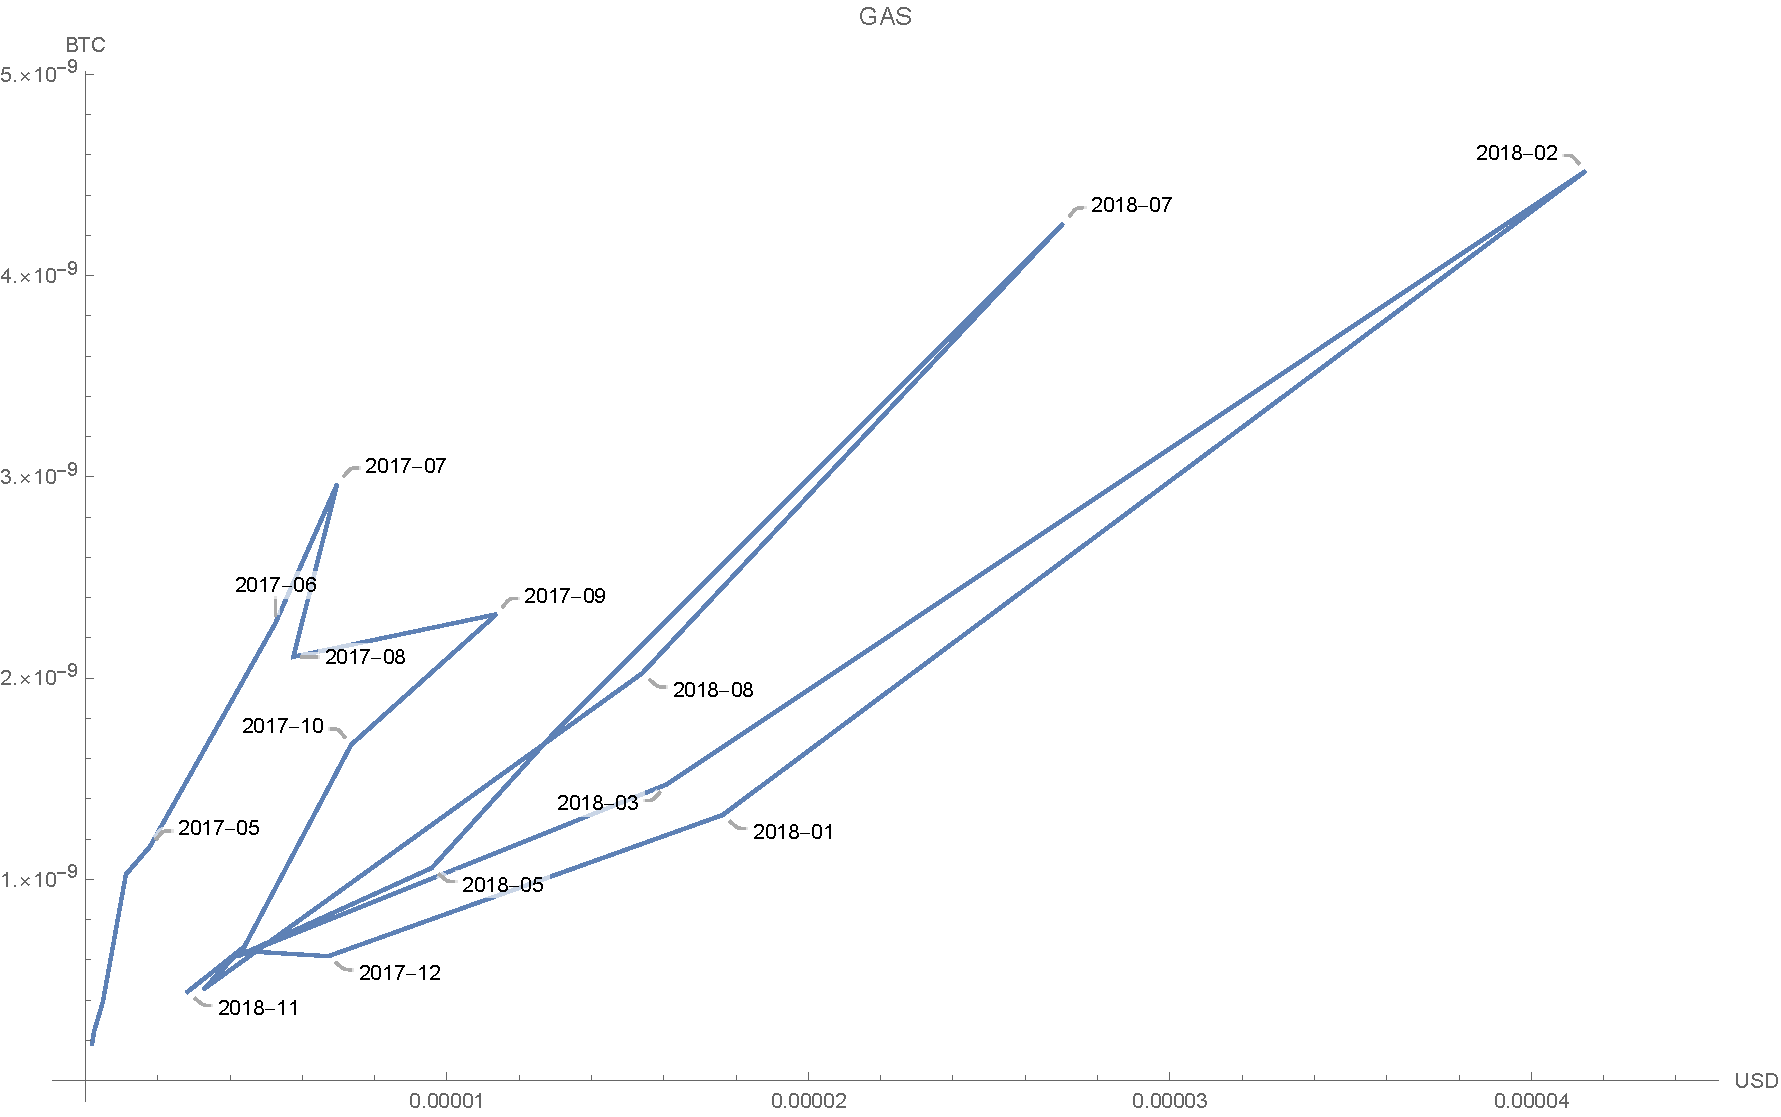
\includegraphics[width=0.45\textwidth]{figures/gas.pdf}\label{fig:gas1}}
	\hfill
	\subfloat[Gas with respect to ETH and Electricity price]{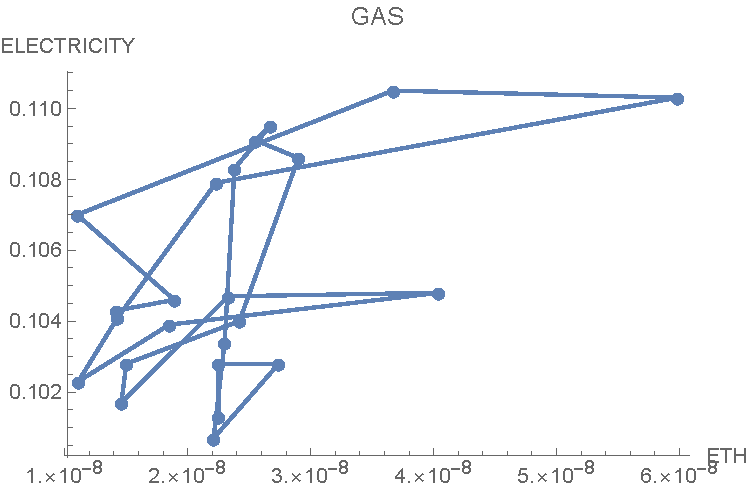
\includegraphics[width=0.45\textwidth]{figures/gasElectricity.pdf}\label{fig:gas2}}
	\caption {Ethereum average GasPrice chart. As mentioned in the Section~\ref{sec:GasInvs}, the two spikes in the chart represent specific events happened in certain dates which have increased the GasPrice.}
	\label{fig:Gas}
	
\end{figure}

%========================%




\textblue{ it would be nice to have a chart : Ether, Electricity (Global energy index), and Gas} \par
Our analysis in Section~\ref{sec:Intro} shows that cryptocurrencies exhibit less stable behavior compared to fiat currencies. Hence, we aim to analyze the price stability of \emph{Gas}. In Ethereum blockchain, every transaction contains a number of operations and there is a precise amount of gas unit associated with each.\footnote{http://ethdocs.org/en/latest/contracts-and-transactions/account-types-gas-and-transactions.html\#what-is-gas} Since Ether is volatile, this concept is introduced to have fixed cost for operations. Thus, even though the price of Ether changes, the amount of Ether corresponding to a unit of gas decreases; so that users pay the same price for the transactions on the Ethereum blockchain. Hence, the notion of gas is yet to be investigated to find out whether it exhibits behavior similar to fiat currencies or cryptocurrencies.

%========================%

%\begin{figure}[!htb]
%	\centering
%	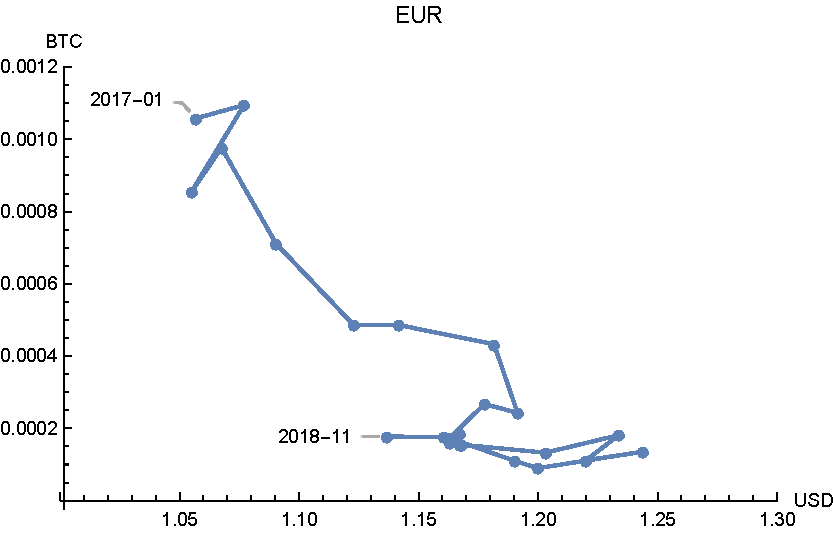
\includegraphics[width=0.95\textwidth]{figures/eur.pdf}
%	\caption{\label{fig:eur} EUR with respect to BTC and gold.}
%\end{figure}
%========================%

%\begin{figure}[!htb]
%	\centering
%	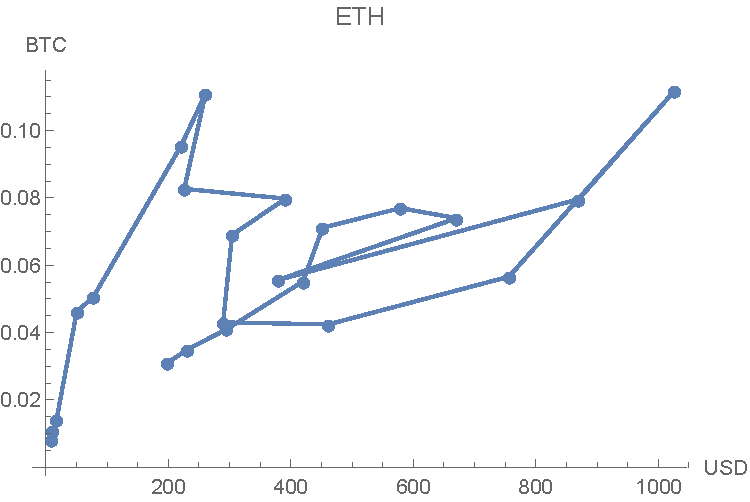
\includegraphics[width=0.95\textwidth]{figures/eth.pdf}
%	\caption{\label{fig:eth} ETH with respect to BTC and gold.}
%\end{figure}
%========================%

%\begin{figure}[!htb]
%	\centering
%	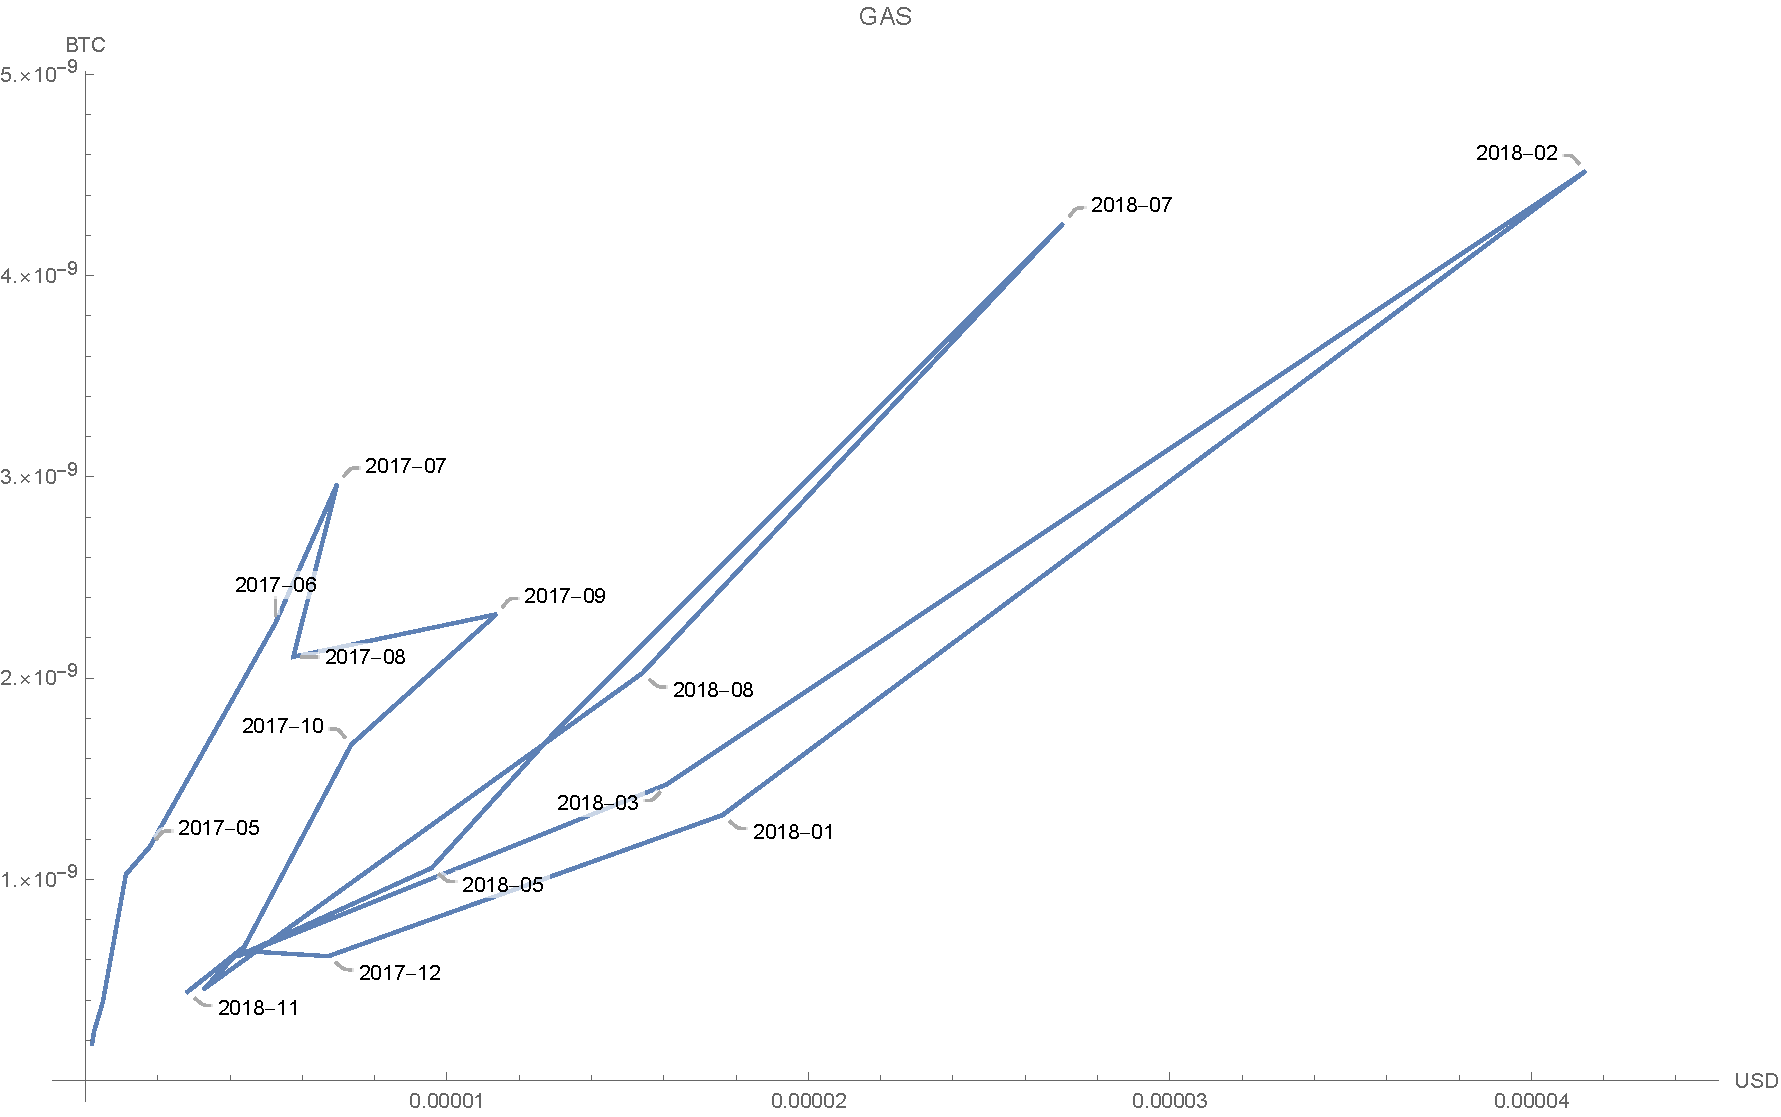
\includegraphics[width=0.95\textwidth]{figures/gas.pdf}
%	\caption{\label{fig:gas} Gas with respect to BTC and gold.}
%\end{figure}
%========================%

%references to figures wrong now!

Figures~\ref{fig:eur}-~\ref{fig:gas} illustrate how the values of EUR, ETH and Gas change with respect to BTC and gold. EUR plot in Figure~\ref{fig:eur} tends to have more movements in the directions 1-5 and 3-7 suggesting that while the value of EUR stays the same according to one axis, it changes according to the other. For instance, between June 2018 and August 2018, the value of EUR increased with respect to BTC, while it stayed the same according to USD. This type of movement suggests that EUR-USD exchange rate is going under less change, whereas BTC-EUR rate is subject to high volatility. On the other hand, in the first half of 2017, while EUR retained its value against BTC, EUR to USD rate went under change.

ETH plot in Figure~\ref{fig:eth} illustrates more volatility against BTC and gold, as there are horizontal, vertical and diagonal changes. The fact that the points are spread in a large range of values indicates drastic changes in ETH price with respect to BTC and Gold.

Compared to Figure~\ref{fig:eur} and Figure~\ref{fig:eth}, gas plot (Figure~\ref{fig:gas}) has mostly diagonal changes, spread over a smaller range. There are less number of changes compared to ETH. Except from the changes between May 2018-July 2018 and January 2018-March 2018, the gas price changes in a smaller range. Even though there are fluctuations in the gas price, it can be inferred that gas price is less volatile than ETH. Also, it worths mentioning that gas is changing over a small scale in x-axis (USD), when compared to Ether's plot over the same axis in a larger interval.


%==========================================%
\begin{figure}[!htb]
	\centering
	\subfloat[ETH]{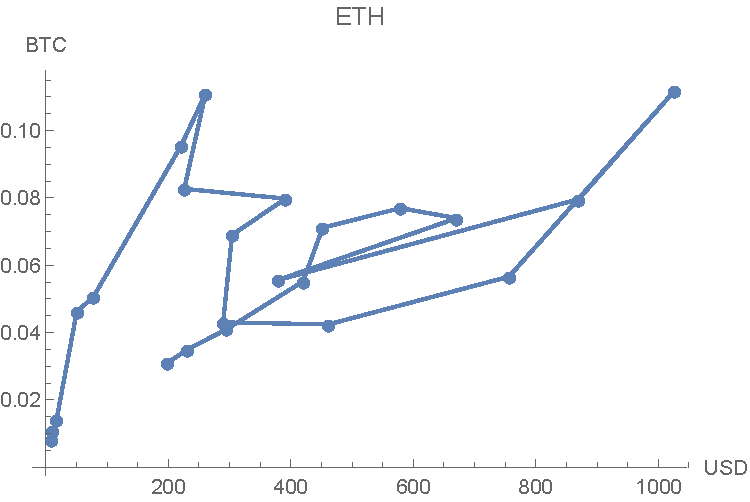
\includegraphics[width=0.45\textwidth]{figures/eth.pdf}\label{fig:cad}}
	\hfill
	\subfloat[XRP]{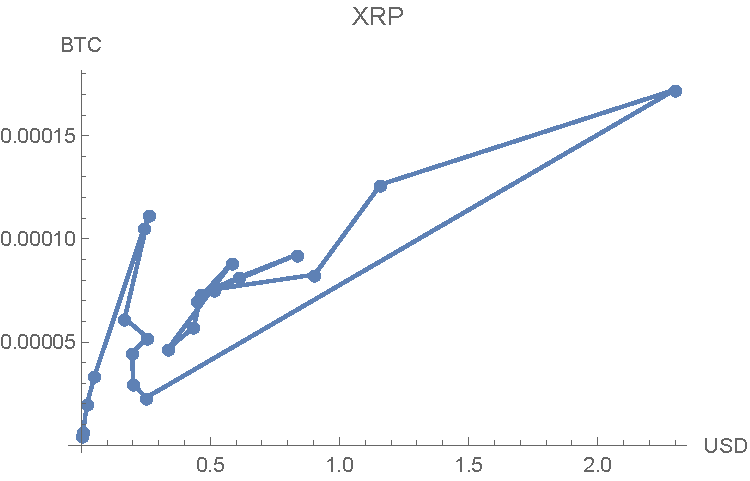
\includegraphics[width=0.45\textwidth]{figures/xrp.pdf}\label{fig:eur}}
	\caption{Volatility in cryptocurrencies}
	\label{fig:fiatandcrypto}
\end{figure}


%========================%

\begin{figure}[!htb]
	\centering
	\subfloat[CAD]{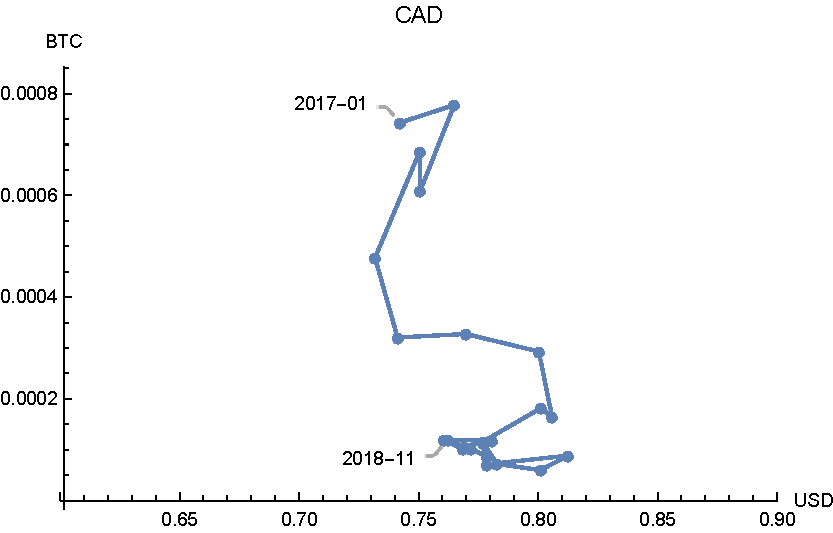
\includegraphics[width=0.45\textwidth]{figures/cad.pdf}\label{fig:cad}}
	\hfill
	\subfloat[EUR]{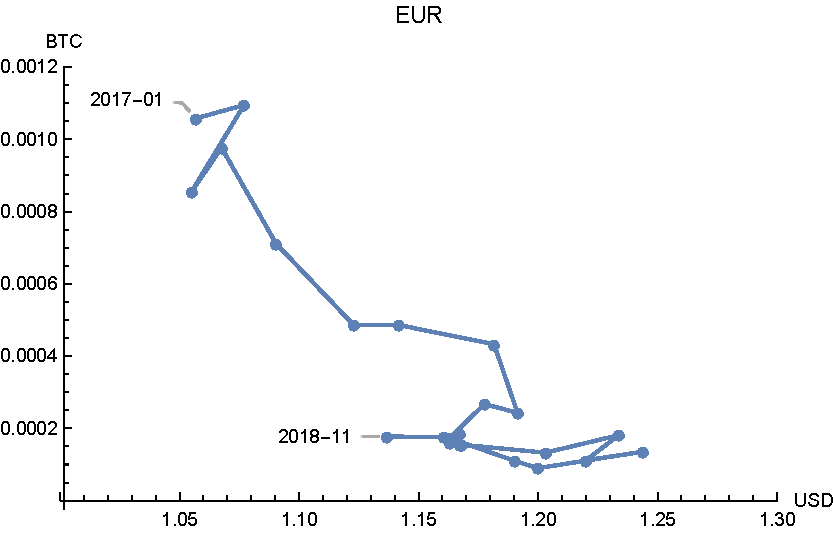
\includegraphics[width=0.45\textwidth]{figures/eur.pdf}\label{fig:eur}}
	\hfill
	\subfloat[Tether]{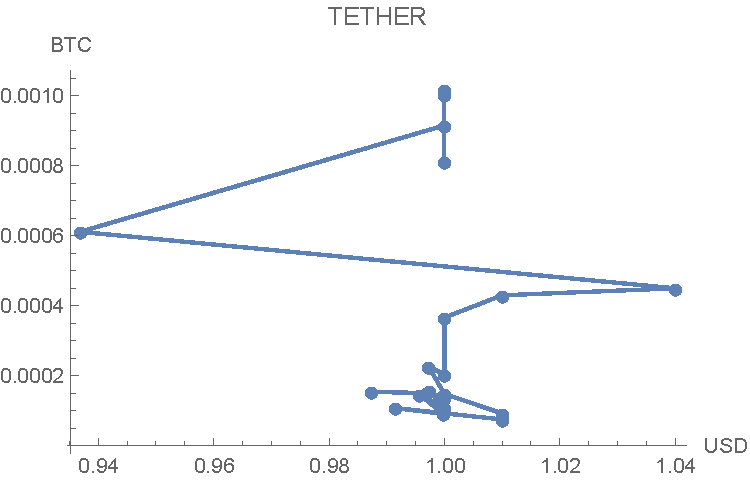
\includegraphics[width=0.45\textwidth]{figures/tether.pdf}\label{fig:tether}}
	\hfill
	\subfloat[BitUSD]{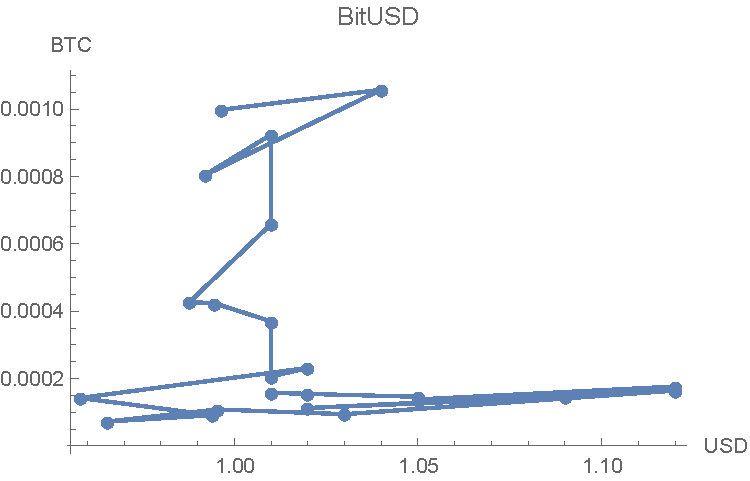
\includegraphics[width=0.45\textwidth]{figures/bitusd.pdf}\label{fig:bitusd}}
	\caption{Stability in fiat currencies and stablecoins }
	\label{fig:fiatandcrypto}
\end{figure}
%========================%

%GRAPHS:
% Figure4: ETH,XRP - (BTC and USD): mostly diagonal movements. Do they move with BTC or not? Shows how cryptocurrencies are volatile. They don't move with BTC
%CAD, EUR,Tether, BitUsd: We expect stablecoins to be close to a vertical line. CAD and EUR are central bank issued "stablecoins" and compared to Tether and BitUsd (crypto stableoins), we can conclude that they are also fairly stable. (same x-axis range!)The graph seems like Tether's having drastic fluctuations. Note that the price change is around 10 cents. The change is accentuated due to the scale.
% TETHER: Does it artificially inflate BTC price? Do they issue un-backed tokens to reinforce BTC price, then sell BTC to fully back tokens?
%TETHER ATTACK: On October 15, 2018, tether, the market dominating stablecoin with a market cap of $2 billion, was attacked, breaking tether’s peg to USD, dropping its value by 7 percent but simultaneously driving up bitcoin and the whole crypto market by more than 10 percent.
%on October 15, 2018; where the price drastically surged from $6,376 at 12.31 UTC to $7,083 at 14.50 UTC. A downturn in price was seen approximately one hour after that to $6,821, before went stable at around $6,400 — $6,600. It was one of the one of the most unexpected fluctuations after a while. The first ‘stable coin’ tether (USDT) which supposedly pegged 1:1 to the U.S. dollar fell up to 15% at the same time as the price of bitcoin fluctuate wildly. The movement caused a loss of trust among traders, causing them to sell tether and invest in other cryptocurrencies. A massive selloff for tether against bitcoin was seen, resulting in a price rise in bitcoin.
%bitcoin and other crypto assets are perfectly negatively correlated with stablecoins.
%speculative attack

% Talk about Ripple surge in  December 2017 {https://www.forbes.com/sites/jessedamiani/2017/12/22/5-reasons-why-the-ripple-price-is-going-up-so-fast-will-the-xrp-surge-continue/#58337c997cbb}  reasons: altcoins gained importance, Rippe's strategy on partnership and customer acquisition, Ripple's partnersips in Asia, rumors that Coinbase will support xrp, "it's speed (4-second transactions) and low fees also make it appealing to general consumers"

\section{Conclusion and Discussion}
In this paper, we analyze the current state of stablecoins with the various options that have been so far proposed to achieve price stability. We also discuss various issues that stablecoins would address. According to the charts represented in the paper, gas is relatively stable in price, while Bitcoin and Ether show volatile behaviour. The reason could be the fact that how users interact with the interface to set the gas price when sending transactions to the Ethereum. By analyzing the properties of gas together with the existing methods to create stablecoin, we can later propose what properties stablecoins should attain.

%==========================================%



